\documentclass[11pt,oneside,a4paper]{report}
\usepackage[utf8]{inputenc}
\usepackage{hyperref}
\usepackage[T1]{fontenc}
\usepackage[danish,english]{babel}
\usepackage{graphicx}
\usepackage[a4paper,margin=2.7cm]{geometry}

\usepackage[sc]{mathpazo} % consider options: osf, sc

\usepackage{amsmath}
\usepackage{amssymb}
\usepackage{amsfonts}
\usepackage{enumerate}
\usepackage{array}

\usepackage{amsthm}
\usepackage{algorithmic}
\usepackage{algorithm}
\usepackage{float}
\usepackage{xcolor}
\usepackage{wrapfig}
\usepackage{subcaption}

\usepackage{tikz,tkz-graph,tkz-berge,tkz-euclide}
\usetikzlibrary{calc,shapes,arrows,backgrounds,fit,positioning}

%\setlength{\parindent}{0pt}
\setlength{\parskip}{2ex} 

\algsetup{linenosize=\large}

\renewcommand{\vec}[1]{\ensuremath {\mathbf #1}}
\newtheorem{thm}{Theorem}[section]
\newtheorem{cor}{Corollary}[thm]
\newtheorem{lemma}[thm]{Lemma}
\newtheorem{definition}{Definition}[section]
\newtheorem{example}[thm]{Example}

%\newcommand{\fitellipsis}[2] % first and second node names without parentheses
%{\draw [red] let \p1=(#1), \p2=(#2), \n1={atan2(\y2-\y1,\x2-\x1)}, \n2={veclen(\y2-\y1,\x2-\x1)}
%	in ($ (\p1)!0.5!(\p2) $) ellipse [x radius=\n2/2+1cm, y radius=0.8cm, rotate=\n1];
%}

%\newcommand{\longfitellipsis}[3] % first and second node names without parentheses
%{\draw [red] let \p1=(#1), \p2=(#2), \n1={atan2(\y2-\y1,\x2-\x1)}, \n2={veclen(\y2-\y1,\x2-\x1)}
%	in ($ (\p1)!0.5!(\p2) $) ellipse [x radius=\n2/2+1cm, y radius=0.8cm, rotate=\n1];
%}

\floatname{algorithm}{Procedure}
\renewcommand{\algorithmicrequire}{\textbf{Input:}}
\renewcommand{\algorithmicensure}{\textbf{Output:}}

\newcommand{\alggoto}[1]{\textbf{goto} \autoref{#1}}

\newcommand{\alginput}[1]{\hspace*{\algorithmicindent}\algorithmicrequire{#1}}
\newcommand{\algoutput}[1]{\hspace*{\algorithmicindent}\algorithmicensure{#1}}
\newcommand{\algio}[2]{
	\alginput{#1}\\
	\algoutput{#2}
}

\newcommand{\setalglineno}[1]{%
  \setcounter{ALC@line}{\numexpr#1-1}}

\begin{document}

\begin{titlepage}
	\begin{center}
		\vspace*{1cm}
		\huge{Structural Properties of Decomposable Digraphs}
		
		\vspace*{0.5cm}
		\large{by}
		
		\vspace{0.5cm}
		\Large{Gabriella Juhl Jensen}
		
		\vspace*{0.5cm}
		\normalsize{supervised by}
		
		\vspace{0.5cm}
		\large{Prof. Jørgen Bang-Jensen}
		
		\vfill
		
		\vspace*{0.7cm}
		\includegraphics[width=0.4\textwidth]{sdulogo}
		
		\vspace*{1cm}
		\MakeUppercase{University of southern Denmark}
		
		\vspace*{0.3cm}
		\MakeUppercase{Department of mathematics and computer science}
		
		\vspace*{0.3cm}
		\large{}
	\end{center}
\end{titlepage}
\tableofcontents
	\section{Introduction}
	Why we need graphs.
	\part{Introduction to Decomposable digraphs and some solutions to Hamilton cycle problem on those digraphs.}
	
\chapter{Notation and Graph Classes}
This chapter introduces graphs and notation. 
Notation in this thesis may diverge from the notation of some articles to ensore a uniform notation.  \autoref{sec:class} introduces names and nottions of graph-classes that will be explored throughout this thesis.
\label{chap:intro}
\section{Graphs and Digraphs}
\label{sec:digraph}
Before going deep into structural properties of decomposable digraphs we first need to establish what a graph is.
For some graph $G(V,E)$ where $V$ and $E$ are two sets contaning the vertices (also commonly called nodes) and egdes of the graph respectivlely.
%Example $V=\lbrace a,b,c \rbrace$ then $a,\ b$ and $c$ are three distinct vertices of the graph $G$ and the only vertices of $G$.
We denote the \textbf{size} of the graph as the number of vertices in the graph $|V|$ this is also known as cardinality of $V$.
In the case of the example the size of $G$ $|V|=3$ it is also called the order of a graph.
An edge $e \in E$ where $e \equiv (a, b)$ and $\{ a, b \} \subseteq V$ is describe by the the two vertices it is connected to $e=(a,b)$.
Thus $(a,b)$ is an edge between the vertex $a$ and $b$.
If an edge goes from and to the same vertex $(a,a)$ it is called a loop.
so the set of edges is describe whit $E=\lbrace (a,b),(a,a),(c,a),(c,b),(c,b)\rbrace$.
The describe example can be seen in figure \autoref{fig:graph}.
If we instead og an edges makes arcs we call it a digraph here the first vertex mentioned in an arc is the vertex from where the arc starts, the second is where the arc is going.
So the arc $(a,b)$ goes from $a$ to $b$, if you wanted it the other way around the arc is $(b,a)$.
these graph contaning only arcs and no edges is called a digraph which is what we in this project are focusing on.\\
\begin{figure}[!h]
    \centering
    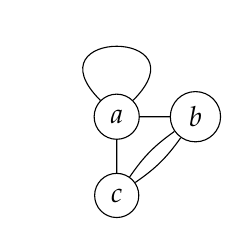
\begin{tikzpicture}
        [main/.style ={draw,circle}]
        \node[main] (a){$a$};
        \node[main] (b)[right of = a]{$b$};
        \node[main](c)[below of= a]{$c$};
        \draw (a) to (b) (c) to (a) (c) to [bend right =10](b) (c) to [bend left =10](b); 
        \draw (a) to [loop] (a);
    \end{tikzpicture} 
    \label{fig:graph}
    \caption{graph $G(V,E)$ used as an example of describing graphs in general}
\end{figure}


before delving into graphs and digraphs we must establish some important prerequisite and properties. 
A graph is simple is there is no loops and no multiple edges. 
With multiple edges it means multiple edges between the same pair of vertices.
A graph is called complete if there for all pair of vertices in the graph is an edge between them.\\
A graph is connected if there exists a path between all pair of vertices in the graph and disconnected otherwise.
a path in a graph is is a walk where a vertex is only passed onces.
A walk in a graph is a ordering of vertices an edges in the graph where the edge in between the vertex in the ordering is an edge between the vertices so for $a,e_1,b$ to be a walk the edge $e_1$ has to be between $a$ and $b$.

in a digraph a graph we have something called the underlying graph. 
An underlying graph of a digraph is where all arcs are replaced by edges (edge is used every time we talk about undirected edges between vertices, when direction is mentioned it is called an arc).
A digraph is connected if the underlying graph is connected, (also called weakly connected), a digraph can be strongly-connected and semi connected too.
A digraph is called semi connected if there for each pair $u$ and $v$ exists a path from either $u$ to $v$ or $v$ to $u$. 
It is said to be strongly connected if for each pair of vertices $u$ and $v$ there exists a path from both $u$ to $v$ and $v$ to $u$.

We can use these to describe som specific collection of graphs as the graph tournaments.
tournaments is a digraph where the underlying graph is complete. 
An underlying graph of a digraph is where all arcs are replaced by edges (edge is used every time we talk about undirected edges between vertices, when direction is mentioned it is called an arc).
So a complete graph of order 5 any orientation of the edges concludes in a tournament.
If instead of replacing the one edge by one arc in either direction, but instead replace it by two arcs the digraph is called semicomplete.

The reason for grouping the digraphs into smaller collections of digraphs (like tournaments is a smaller collection of semicomplete digraphs) is because of problems is easy describe on specific graphs than general graphs.

We have these graph called NP-hard problems which sometimes sound easy solvable for graphs but only for some specific graphs we know how to solve it in polynomial time. 
\begin{definition}
    define NP-hard problems
\end{definition}

In this paper we focusing on the specific digraphs that are decomposable. 
A decomposable digraph is a digraph $D=H[G_1,G_2,\dots,G_|H|]$ where each $G_i$ is disconnected graphs replacing each vertex of the digraph $H$. ...

\section{Computational complexity}
\label{sec:complexity}
In this section we will go over how time is measured for an algorithm and what it means for a problem to be polynomially solveable or polynomially verifyable. Also what it means for a problem to be NP-hard and NP-complete and how we found out if a problem is either of them. 

\subsection{Measure time of algorithm (Polynomial, exponential)}
The runing time of an algorithm is based on how many steps it is going thourgh which is somtimes based on the input that the algorithm takes we are going to denote an algorithms running time as a function $f(n)$ over the input $n$. 
This is how different functions can descirbe the running time of an algorithm, if an algorithm has the same number of steps no matter what the input is it has a constat running time where the constant is the number of steps the algorithm uses. 

An algorithm can also take the form of an polynomial function or even exponentiel, if this is the case we uses some notation as big-$O$ notation or $\theta$. 
Big-oh is the most used one and is the notation we are going to use in this thises, if the algorithm takes $f(n)=4n^3 +2n^2-n+2$ time we denote it in big-oh notation as $O(n^3)$ as it is the biggest term of $f(n)$.  

Since the shorter the runningtime is the better the algortihm is.
Since the exponentiel runningtime algortihms take forever on large inputs, we would want to improve them, but sometimes you are left with problems where that is not a possibility.

So we are going to classify the problems in gruops of how long time it take to decide or verify the problems solution. a problem that is decided i polynomiel time is in the class called $P$.
Which means for every given time of input in a problem from \textbf{P} we can find the solution for the problem in polynomiel time.

\subsection{NP problems and classifications}
As shortly described above there is something called a \textbf{polynomial verifier} for a problem. 
That means given a problem and then given a solution we can in polynomial time verify if it is a solution to the given problem. This is the class we call NP.
\begin{definition}
    \textbf{NP} is the class of languages that have polynomial time verifiers.
\end{definition}

Obiously if you can find a solution in polynomial time you can also verify whether a solution is correct in polynomial time. 
So $P\subseteq NP$. 
There is also a class called $NP-Hard$ but before we can explain that we need to explain what it means for a problem to be polynomial reduceable to another problem. 
For a specific problem $A$ and another problem $B$ then if there exists an algorithm that can take a solution from $A$ and make it a solution for $B$ in polynomial time. 
When such a algorithm exists it is called a polynomial verifier and we say that $A$ is \textbf{polynomial reducable} to $B$ or just that $A$ is \textbf{reduced} to $B$. 
\textbf{NP-Hard} are the class of problems that every NP problem can be polynomiel reduced to. 
A problems in the class of NP-Hard problems does not nessesarily mean that it is NP it-self.
If a problem is both \textbf{NP} and \textbf{NP-Hard} we call it \textbf{NP-Complete}. 
The problems we are \textcolor{red}{mostly} focusing on is in the class of \textbf{NP-Complete} problems.   

\section{Classes of Digraphs}
\label{sec:class}
A \textbf{Tournament} is a digraph in which the underlying graph is complete. 
So in a complete graph of order 5, any orientation of the edges concludes in a tournament.
Strong digraphs are also in themselves a classification of digraphs. 
Classes of digraphs can overlap each other or fully contained in each other, like tournaments is fully contained in the class called semicomplete digraphs.
A \textbf{semicomplete} digraph is where the underlying graph is a complete multigraph, there can be some multiple edges in between the same pair of vertices in the underlying graph (parallel edges). 
Since the class called semicomplete digraphs contains all digraphs where the underlying graph is a complete multigraph, it clearly also contains the graph with only one arc between every pair of vertices (Tournaments).
A digraph is \textbf{complete} if for every pair of vertices $a,b\in V$, the arc $(a,b)$ and $(b,a)$ are present in the graph. \\
If you can split the vertices of a graph $V$ into two sets of vertices $A$ and $B$ such that $A\cup B=V$, and there are no arcs inside these sets, then we classify this as an \textbf{bipartite} digraph. 
This means all arcs in the graph are in the form $(a,b)$ or $(b,a)$ for all $a\in A$ and $b\in B$. 
The sets $A$ and $B$ are called the partites of $D(V,A)$. 
The underlying graph of a bipartite digraph is also called bipartite since there are no edges inside $A$ or $B$.
%If there exists more then two of these partite sets we call the digraphs \textbf{multipartite}, since there is multiple partite sets in the graph, bipartite sets $\subset$ multipartite. \\
A much used type of digraph is an \textbf{acyclic} digraph. 
It is a digraph where there exists an ordering of the vertices $V={v_1, v_2,\dots , v_n}$ where the arcs in the digraph are $(v_i, v_j)$ where $i<j$ for all $(v_i, v_j)\in A$. 
This ordering is called an \textbf{acyclic ordering}, and there can be many of these orderings in the same digraph.
This ordering can also be used to order strong components in a non-strong digraph, such that the ordering of the components $C_1,C_2,\dots C_k$ is an acyclic digraph when contracting the components into $k$ vertices. 
When classifying digraphs, there are several ways of doing this, like \textbf{transitive} digraphs which are digraphs where for all vertices $a,d,c\in V$ where the arc $(a,b)$ and $b,c$ is present in the digraph ($\in A$), the arc $(a,c)$ has to be a part of $A$ too. 
Using the same kind of classification, there are digraphs which are \textbf{Quasi-transitive}, which is for all vertices $a,d,c\in V$ where the arc $(a,b)$ and $b,c$ is present in the digraph ($\in A$, $a$ and $c$ has to be adecent by at \textit{least} one (more arcs in between are also allowed) arc in either direction ($(a,c)$ or $(c,a)$)). These graphs are going to be mentioned a lot in this thises since the graph is also what we call \textbf{decomposable}.\\
A \textbf{Decomposable} digraph $D=S[H_1,H_2,\dots H_s]$ is a digraph $D$ that can be decomposed into $H_1,H_2, \dots , H_s$ \textbf{houses} and a digraph $S$ denoted as the \textbf{quotient} digraph where $|V(S)|=s$. 
Let $S$ be the quotient digraph of $D$ where $V(S)=\lbrace s_1,s_2,\dots,s_s\rbrace$. 
If each $s_i$ is replaced by the digraph $H_i$ $i=1,2,\dots,k$, we have the digraph $D$, where $H_i\rightarrow H_j \in D$ if $s_i\rightarrow s_j\in S$. 
This is called a \textbf{composition} of $S$ or a \textbf{decomposition} of $D$.
This is the class of digraphs we are focusing on in this thesis. 
If all the houses are independent sets, we call $D=S[H_1,H_2,\dots ,H_k]$ the extension of $S$. 
If $S$ is a semicomplete digraph, we call the extension of these \textbf{extended semicomplete} digraph.
Like we already mentioned, Quasi-transitive digraphs are decomposable but we have several classes that are decomposable, and another class of digraphs that we are giong to cover in this dissertation are \textbf{locally semicomplete} digraphs.\\
First, we introduce \textbf{locally in-semicomplete} digraphs where for every in-neighboor of a vertex, $x\in V$ has to be adjacent. 
This has to be true for all $x\in V$ ($x\cup N^-(x)$ induces a semicomplete digraph $\forall x\in V$). 
When $x\cup N^+(x)$ for all vertices in $D$, it classifies as \textbf{locally out-semicomplete} digraphs. 
Respectively, it is called an out-locally semicomplete digraph if $\forall x\in V$, $N^+(x)$, has to be adjacent. 
If a digraph is both locally in-semicomplete and locally out-semicomplete, it is called a \textbf{locally semicomplete} digraph. 
Why both quasi-transitive digraphs and some locally semicomplete digraphs are decomposeble will be described in \autoref{sec:gdecomposable}.\\
The last class of digraph that are important for this thesis are the round digraphs. 
A digraph is called a \textbf{round} digraph if there exists an ordering of the vertices $v_1,v_2,\dots,v_n$ such that for all $v_i$, $N^+(v_i)={v_{i+1},v_{i+2},\dots ,v_{i+d^+(v_i)}}$ and $N^-(v_i)={v_{i-d^-(v_i)},v_{i-(d^-(v_i)-1)},\dots ,v_{i-1}}$.






\chapter{Decomposable Digraphs}
\label{chap:decomposable}
Decomposable digraphs is what we in this thesis is focusing on. 
We have introduced short what a decomposable digraph is but there is subclasses to focus on and a lot of other crucial definitions and theroems to cover about these digraphs before delving into the NP-hard problems. 
First we cover some general things about decomposable digraphs the next section is about quasi-transitive digraphs, and why they are a subclass of decomposable digraphs and $\phi_1$-decomposable digraphs. At the end of the section we prove that these decompositions can be found in polynomial time. 
Which is going to be crucial for solving some NP-hard problems for this class of digraphs. Then we are going to look at a very general class of digraphs locally semicomplete digraphs, where this class can be split up to 3 different subclasses where 2 of those are decomposable. 
This is covered in \autoref{sec:locally} and is going to be used in later chapthers. 
\section{General about Decomposable digraphs}
\label{sec:gdecomposable}
Recall that a decomposable digraph $D=S[H_1,H_2,\dots H_k]$ can be decomposed into a main graph $S$ (also sometimes called \textbf{quotient} graph), where $|S|=k$ and $k$ houses $H_1,H_2,\dots , H_k$, where each vertex in $S=\lbrace v_1,v_2\dots ,v_k\rbrace$ is replaced by the house ($H_i$ replaces $v_i$).
The arcs between the houses are as follows: $H_i \rightarrow H_j$ in $D$ if $v_i\rightarrow v_j$ in $S$. 
Remember that for a set $X$ to dominate another set $Y$ (meaning every vertex in the dominating set dominates every vertex in the dominated set), we denoted it $X \rightarrow Y$. 
If no arc between $v_a$ and $v_b$ is in $S$, then there is no arc between the sets $H_a$ and $H_b$ in $D$. 
A nice property of decomposable digraphs is that if there is an arc between $H_i$ and $H_j$, either one of the houses totally dominates the other (ex. $H_i \Rightarrow H_j$) or they dominate each other (ex. $H_i \rightarrow H_j$ and $H_j\rightarrow H_i$).

\noindent Decomposable digraphs can be classified by a set of digraphs $\phi$. 
When $D=S[H_1,H_2,\dots ,H_k]$ it is \textbf{$\phi$-decomposable} if $D\in \phi$ or if $S\in \phi$. 
The chioces of $H_i$ for $i=1,2\dots , k$ does not determine anything about the digraph being $\phi$-decomposable, but the class of \textbf{totally $\phi$-decomposable} digraphs is where $D$ is $\phi$-decomposable and each $H_i$ is totally $\phi$-decomposable. 
We are going to make two such sets of digraphs: $\phi_1$, which is the union of semicomplete digraphs and acyclic digraphs both classes described in \autoref{sec:class} and $\phi_2$, which is the union of semicomplete and round digraphs also described in \autoref{sec:class}.  
\begin{align}
    \phi_1=\lbrace \text{Semicomplete digraphs}\rbrace\cup \lbrace \text{Acyclic digraphs}\rbrace
    \label{eq:phi1}\\
    \phi_2=\lbrace \text{Semicomplete digraphs}\rbrace\cup \lbrace \text{Round digraphs}\rbrace
    \label{eq:phi2}
\end{align}

Take these sets $\phi_1$ and $\phi_2$. 
Then for every induced subdigraph of a digraph $D$ where either $D\in \phi_1$ or $D\in \phi_2$, then the induced digraph is in the same set (so if $D\in \phi_1$ the induced subdigraph is in $\phi_1$, same goes for $\phi_2$).
When this is true for a set $\phi$, the set is called \textbf{hereditary}. So both $\phi_1$ and $\phi_2$ are hereditary.
\begin{lemma}
    Let $\phi$ be a hereditary set of digraphs. If a given digraph $D$ is totally $\phi$-decomposable, then every induced subdigraph $D'$ of $D$ is totally $\phi$-decomposable.
    \label{lemma:hereditary}
\end{lemma}
It also turns out that for $\phi_1$ and $\phi_2$, there exists an algorithm that checks whether a digraph $D$ is totally $\phi_i$-decomposable ($i=1,2$).
\begin{thm}~\cite{banggutin}
    There exists an $O(n^2m+n^3)$-algorithm for chekking if a digraph with $n$ vertices and $m$ arcs is totally $\phi_i$-decomposable for $i=1,2$.
    \label{thm:phipoly}
\end{thm}
\noindent $O(n^2m+n^3)$ is clearly a polynomial algortihm. 
\section{Quasi-transitive Digraph}
\label{sec:quasi}
First we need to recall what a quasi transitive digraph is. 
For every triplet $x,y,z$ in a quasi-transitive digraph if $x\rightarrow y$ ($x$ dominates $y$) and $y\rightarrow z$ ($y$ domitaes $z$), then there has to be at least one arc in either dirction between $x$ and $z$. Quasi-transitive digraphs can be decomposed no matter if there are strong or nonstrong digraphs. 
\begin{thm}\cite{bangJGT85}
    Let $D$ be a quasi-transitive digraph.
    \begin{enumerate}
        \item If $D$ is not strong, then there exists a transitive acyclic digraph $T$ on $t$ vertices and strong quasitransitive digraphs $H_1,\dots,H_t$ such that $D=T[H_1,\dots,H_t]$.
        \item If $D$ is strong, then there exists a strong semicomplete digraph $S$ on $s$ vertices and quasitransitive digraphs $Q_1,\dots ,Q_s$ such that each $Q_i$ is either a single vertex or is nonstrong and $D=S[Q_1,\dots,Q_s]$.
    \end{enumerate}
    \label{thm:quasidecom}
\end{thm}
\begin{proof}
    blablabla
\end{proof}
From this theorem we can see that quasi-transitive digraphs is totally $\phi_1$-decomposable. 
Since the transitive digraph for the nonstrong quasi-transitive digraphs is acyclic $T\in \phi_1$ and each $Q_i$ is in itself strong quasi triansitive digraphs and you can therefore use \autoref{thm:quasidecom} agian.  
For the strong quasi-transitive digraphs $D$, $S$ is semicomplete so $S\in \phi_1$ and each $Q_i \in \phi_1$ because it is either one vertex which is a digraph that is both acyclic and semicomplete or it is non-strong and must be quasi-transitive and therefore \autoref{thm:quasidecom} can be used agian. So every nonstrong and strong quasi-transitive digraphs is totally $\phi_1$-decomposable.

\begin{thm}
    \textcolor{red}{quasi decomposition can be found in poly time}
\end{thm}

\section{Locally semicomplete Digraph}
\label{sec:locally}
blablabla
\begin{thm}
    \textcolor{red}{round decompose locally semicomplete digraph}
\end{thm}
Every locally semicomplete digraph can be classified into some other groups of digraphs namely semicomplete digraphs and round decomposable digraphs and the last one which is neither of the two is call evil. Round decomposable digraph $D=R[D_1,\dots,D_r]$ is where $R$ is a round digraph of the strong componentents $D_i$ and $|R|=r$.
\begin{thm}~\cite{bangJGT85}
    Let $D$ be a locally semicomplete digraph. Then exactly one of the following possibilities holds. Furthermore, there is a polynomial algorithm that decides which of the properties hold and gives a certificate for this.
    \begin{itemize}
        \item[(a)] $D$ is round decomposable with a unique round decomposition $R[D_1,\dots ,D_r]$, where $R$ is a round local tournament on $r\geq 2$vertices and $D_i$ is strong semicomplete digraph for $i=1,2,\dots,r$.
        \item[(b)] $D$ is evil 
        \item[(c)] $D$ is a semicomplete digraph thet is not round decomposable. 
    \end{itemize}
\end{thm}
If the locally semicomplete digraph is nonstrong it turns out that it is decomposable this is called a semicomplete decomposition.
\begin{thm}~\cite{bangJGT85,banggutin,bangJCT102}
    Let $D$ be a nonstrong locally semicomplete digraph and let $D_1,D_2,\dots,D_p$ be the acyclic order of the strong components of $D$. Then $D$ can be decomposed into $r\geq 2$ disjoint subdigraphs $D_1',D_2',\dots, D_r'$ as follows:
    \begin{align*}
        D_1'=D_p, \lambda_1=p,\\
        \lambda_{i+1}=min\lbrace j|N^+(D_j)\cap V(D'_i)\neq \emptyset\rbrace,
    \end{align*}
    and
    \begin{equation*}
        D'_{i+1}=D\left<V(D_{lambda_{i+1}})\cup V(D_{lambda_{i+1}+1})\cup \cdots \cup V(D_{lambda_{i}-1})\right>
    \end{equation*}
    The subdigraphs $D'_1,D'_2,\dots,D'_r$ satisfy the properties below:
    \begin{itemize}
        \item[(a)] $D'_i$ consists of some strong components that are consecutive in the acyclic ordering of the strong components of $D$ and is semicomplete for $1=1,2,\dots,r$;
        \item[(b)] $D'_{i+1}$ dominates the initial component of $D'_i$ and there exists no arc from $D'_i$ to $D'_{i+1}$ for $i=1,2,\dots,r-1$;
        \item[(c)] if $r\geq 3$ then there exists no arc between $D'_i$ and $D'_j$ for $i,j$ satisfying $|j-i|\geq 2$  
    \end{itemize}
    \label{thm:semicompletedecom}
\end{thm}
For simplification of \autoref{thm:semicompletedecom} the properties is drawn out in \autoref{fig:properties}
\begin{figure}
    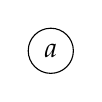
\begin{tikzpicture}[main/.style ={draw,circle}]
        \node[main](a){$a$};
    \end{tikzpicture}
    \caption{(a)(b) and (c)}
    \label{fig:properties}
\end{figure}
Now we focus more on the structure of the evil locally semicomplete digraph which we have not covered jet, there is a fine understanding of the structure of round decomposable and the semicomplete digraphs, even the semicomplete decomposition which is a part of the evil structure too.
First we have to recall what a minimal seperator from \autoref{sec:digraph}, then use this to construct what we call a \textbf{good} seperator.
\begin{lemma}~\cite{bangJGT85}
    Let $S$ ba a minimal seperator of the locally semicomplete digraph $D$. Then either $D\left< S\right>$ is semicomplete or $D\left< V-S\right>$ is semicomplete.
    \label{lem:whichsemicomplete}
\end{lemma}
Then a \textbf{good} seperator of a locally semicomplete digraph is minimal and $D\left<V-S\right>$ is not semicomplete.
When finding a good seperator in a evil locally semicomplete digraph, then the part that is left $D-S$ a semicomplete decomposition can be found it turns out that there is a lot to say about this decomposition.
\begin{thm}~\cite{bangJGT85,bangJCT102}
    Let $D$ be an evil locally semicomplete digraph then $D$ is strong and satisfies the following properties.
    \begin{itemize}
        \item[(a)]There is a good seperator S such that the semicomplete decomposition of $D-S$ has exactly three components $D'_1,D'_2,D'_3$ (and $D\left<S\right>$ is semicomplete by \autoref{lem:whichsemicomplete});
        \item[(b)] Furthermore, for each such $S$, there are integers $\alpha, \beta,\mu,\nu$ with $\lambda_2\leq \alpha \leq \beta \leq p-1$ and $p+1\leq \mu \leq \nu \leq p+q$ such that 
        \begin{align}
            &N^-(D_\alpha)\cap V(D_\mu)\neq \emptyset \text{and} N^+(D_\alpha)\cap V(D_\nu)\neq \emptyset,\\
            \text{or} &N^-(D_\mu)\cap V(D_\alpha)\neq \emptyset \text{and} N^+(D_\mu)\cap V(D_\beta)\neq \emptyset,
        \end{align} 
        where $D_1,D_2,\dots, D_p$ and $D_{p+1},\dots,D_{p+q}$ are the strong decomposition of $D-S$ and $D\left< S\right>$, respectively, and $D_{\lambda_2}$is the initial component of $D'_2$ 
    \end{itemize}
    \label{thm:evildecom}
\end{thm}
Even though this is a structure we can work with, we can actually go deeper into the structure of this evil locally semicomplete digraph. Namly trying to group the components inside the semicomplete decomposition $D'_1,D'_2,D'_3$ and the good seperator $S$. This structer is menation in \cite{bangJGT85} but also in \cite{tildeDMCS}. First we can establish this lemma which is a big part of the structure of evil locally semicomplete digraphs.
\begin{lemma}~\cite{tildeDMCS}
    Let $D$ be an evil locally semicomplete digraph and let $S$ be a good seperator od $D$. Then the following holds:
    \begin{itemize}
        \item[(i)] $D_p\Rightarrow S\Rightarrow D_1$.
        \item[(ii)] If $sv$ is an arc from $S$ to $D'_2$ with $s\in V(D_i)$ and $v\in V(D_j)$, then 
        \begin{equation*}
            D_i\cup D_{i+1}\cup \dots D_{p+q}\Rightarrow D_1\cup\dots \cup D_{\lambda_2-1}\Rightarrow D_{\lambda_2}\cup \dots \cup D_j
        \end{equation*}.
        \item[(iii)] $D_{p+q}\Rightarrow D'_3$ and $D_f\Rightarrow D_{f+1}$ for $f\in [p+q]$, where $p+q+1=1$.
        \item[(iv)] If there is any arc from $D_i$ to $D_j$ with $i\in [\lambda_2-1]$ and $j\in [\lambda_2,p-1]$, then $D_a\Rightarrow D_b$ for all $a\in [i,\lambda_2-1]$ and $b\in[\lambda_2,j]$.
        \item[(v)] If there is any arc from $D_k to D_l$ with $k\in [p+1,p+q]$ and $l\in [\lambda_2-1]$, then $D_a\Rightarrow D_b$ for all $a\in [k,p+q]$ and $b\in [l]$.   
    \end{itemize}
\end{lemma}


\chapter{Path cover and hamilton cycles}
\label{chap:hamilton}
In this chapter the focus is the hamilton cycle problem, where we know that if we can solve the path covering problem then we can solve the hamilton cycle problem for quasi-transitive digraphs.\\
In the first section we are going to cover, what a hamilton path is, and a hamilton cycle Since these to problems are well know as \textbf{NP-Complete} which will shortly be introduced too.\\
The next section is about path-mergeable digraphs and that locally semicomplete digraphs are a subclass of these and how this helps in the path covering problem and hamilton cycle problem. 
%Then state some theorems that says knowing special things about the graph we know when it contain a hamilton cycle. \\
The following section is covering quasi-transitive digraphs and whether or not there exists a hamilton cycle in those. Here the decomposition of the quasi-transitive digraphs is going to be a crucial part of proving this. \\


\section{The Hamilton Path and Cycle Problem}
\label{sec:hNP}
The Hamilton cycle problem in a digraph is well known, but here is a short explanation of what that is.
When we define what a Hamiltonian digraph is, we first have to explain what a Hamilton cycle is. 
A Hamilton cycle is a directed cycle $C_H$ in a digraph that contains every vertex in the digraph $\forall v\in V(D),\ v\in C_H$.\\
\begin{definition}
    A Hamiltonian digraph is a graph containing a Hamilton cycle. 
\end{definition} 
We can also define digraphs called traceable digraphs:
\begin{definition}
    A traceable digraph is a digraph containing a Hamilton path.
\end{definition}
A Hamilton path is a path containing all vertices of the digraph.\\
It is NP-complete to find out whether an arbitrary given digraph is traceble or Hamiltonian.
Before going into why the problems are NP, we are going to state some obvious conditions for graphs to be traceable or Hamiltonian. \\
For a digraph to be traceable, it needs to be semi-connected, and for a digraph to be Hamiltonian, it needs to be strong. Since a Hamilton cycle is a cycle factor in a digraph $D$ hence a condition for a digraph to be Hamiltonian is that it need to contain a cycle factor.\\
This is all explained and proven in the book 'Digraph', written by Bang-Jensen and Gutin \cite{banggutin}. 
%We are going to show (shortly explain) why the Hamilton path problem is \textcolor{red}{NP-Hard} by reducing a problem we know is NP to the Hamilton path problem.
%Then we are going to show that if we know that a digraph is traceable it takes polynomial time to figure out wheter it is Hamiltonian too, making the traceable problem \textcolor{red}{NP-Hard} too.
%Because if we in polynomial time could figure out wheter a arbitrary digraph is traceable you know that if it is not, it is defenatly not Hamiltonian. 
%And if it is you can in polynomial time figure out if it is Hamiltonian, making the hamton cycle problem a polynomial time solution problem (not \textcolor{red}{NP-Hard}).
%\begin{thm}
%    Finding out wether a digraph is trecable is a NP-Hard Problem
%\end{thm}
%\begin{proof}
%    sketz \textcolor{red}{blbalbalbalablabala}
%\end{proof}

%\begin{thm}
%    Finding out wether a digraph is Hamiltonian is a NP-Hard Problem
%\end{thm}
%\begin{proof}
%    sketz \textcolor{red}{blbalbalbalablabala}
%\end{proof}
\section{Hamiltonian Locally semicomplete Digraphs}
\label{sec:hlocally}
Recall that a locally semicomplete digraph is both in-locally semicomplete and out-locally semicomplete. 
Before this gets relevant we are going to introduce a class of digraphs called path-mergeable they are not introduced under section \autoref{sec:class} since we are only going to use it in this section.
A short explanaition of a path mergeable digraph is that it is the class of digraphs where given two paths with the start- and endpoint incommen you can merge the two paths into one using all vertices in the two paths. 
A more formal definition of path mergeable digraphs is if there exists a pair of distinct vertices $x,y\in V(D)$ and any two disjoint $(x,y)$-paths there exists a new path from $x$ to $y$ where it is a union of the vertices used in the two vertex-disjoint paths (ending up with a "merge" path of the two given path).\\
These digraphs are easy to regonize with the following corolary we can do it in polynomial time too and the following theroem gives us a nice propertie of path-mergeable digraphs.
\begin{cor}~\cite{banggutin}
    Path-mergeable digraphs can be regonized in polynomial time
\end{cor}
\begin{thm}~\cite{banggutin}
    A digraph $D$ is path mergeable if and only if for every pair of distict vertices $x,y\in V(D)$ and every pair $P=xx_1\dots x_ry,\ P'=xy_1\dots y_sy$, $r,s\geq 1$ of internally disjoint $(x,y)$-paths in $D$, either there exists an $i\in \lbrace 1,\dots ,r\rbrace$, such that $x_i\rightarrow y_1$, or there exists a $j\in \lbrace 1,\dots, y_j\rightarrow x_1\rbrace$.
    \label{thm:pathmerge}
\end{thm}
to explain this \autoref{thm:pathmerge} it tells us that for every path mergeable digraph in every two disjoint $(x,y)$-path there has to be from one of the path a vertex that dominates the first vertex after $x$ in the other path. This has to hold for every distict pair of vertices $x$ and $y$. \\
It turns out that in these digraph we can easily determine whether it is a hamiltonian digraph too.
\begin{thm}
    A path-mergeable digraph $D$ of order $n\geq 2$ is hamiltonian if and only if $D$ is strong and $UG(D)$ is $2$-connected.
    \label{thm:pathham}
\end{thm}
\begin{cor}
    There is an $O(nm)$-algorithm to decide whether a given strong path-mergeable digraph has a hamiltonian cycle and find one if it exists.
    \label{cor:polypath}
\end{cor}
So it turns out that for path-mergeable digraphs this problem is polynomial solveable, and a subclass of these path-mergeable digraph is namely the locally semicomplete digraphs. If we can prove this we only know that we can solve the hamilton cycle in polynomial time and since the locally semicomplete digraphs is a subclass of in-locally semicomplete digraphs we have an even better time for these.
\begin{prop}
    Every locally in-semicomplete (out-semicomplete) digraph is path-mergeable.
\end{prop}
\begin{proof}
    proof this ... ... ... ... ... ... ... 
\end{proof}

Then it turns out that \autoref{thm:pathham} and \autoref{cor:polypath} can be imporved if we are only looking at the in-locally semicomplete digraph, since the locally semicomplete digraph is a subclass of these, and it is the ones we are interested in, in this thises. It turns out that every strong in-locally semicomplete digraph has a 2-connected underlyning graph, which means the only thing we need to check is whether it is a strong digraph.
\begin{thm}
    A locally in-semicomplete digraph $D$ of order $n\geq 2$ is hamiltonian if and only if $D$ is strong.
\end{thm}

It turns out that when looking at the strong locally in-semicomplete digraphs out of the path-mergeable digraph finding the hamiltonian cycle can be done i polynomial time by theorem discorvered by ... ...
\begin{thm}
    There is an $O(m+n\text{log}n)$-algorithm for finding a hamiltonian cycle in a strong locally in-semicomplete digraph.
\end{thm}


\section{Hamiltonian Quasi-transitive Digraphs}
\label{sec:hquasi}
First of all, we have to recall \autoref{thm:quasidecom} since it is the key theorem to solve the Hamilton cycle problem in polynomial time. \\
Remember that a condition for a digraph to be Hamiltonian is that it need to be strong, so for finding a Hamilton cycle in a quasi-transitive digraph, we are not interested in the non-strong digraphs. 
Leaving only the strong quasi-transitive digraphs with decomposition $S[Q_1,\dots Q_s]$ from \autoref{thm:quasidecom}. 
The given decomposition of a strong quasi-transitive digraph has a semicomplete digraph as the quotient. This is why we need some insight to these before the main solution in this subsection can be proven. 
Another composition of semicomplete digraphs is the extension of these, called extended semicomplete digraphs. 
An extension of a digraph is a composition of the given digraph $S$ where the houses of the composition is either a single vertex or independence sets. \\
Before we explain when we can find a Hamilton cycle in strong quasi-transitive digraphs, we need to recall what a cycle factor is. 
From \autoref{sec:digraph}, we shortly explained that a cycle factor is when we can find $C_1,\dots C_k$ cycles in $D$ contaning all vertices of $D$. 
\begin{thm}~\cite{gutinMNN2}
    An extended semicomplete digraph $D$ is Hamiltonian if and only if $D$ is strong and contains a cycle factor. One can check whether $D$ is Hamiltonian and construct a Hamilton cycle of $D$ (if one exsists) in time $O(n^{2.5})$.
    \label{thm:extended}
\end{thm}
\begin{thm}~\cite{bangJGT20}
    A strong quasi-transitive digraph $D$ with a canonical decomposition \\$D=S[Q_1\dots, Q_s]$ is Hamiltonian if and only if it has a cycle factor $\mathcal{F}$ such that no cycle of $\mathcal{F}$ is a cycle of some $Q_i$.
    \label{thm:qhcycle}
\end{thm}
\begin{proof}
    Since a Hamiltonian cycle needs to cover all vertices in a digraph, we know that it must cross every $Q_i$. 
    Moreover the Hamilton cycle is a cycle factor not fully contained in any $Q_i$. 
    So we only need to show that if we have a cycle factor $\mathcal{F}$, where no cycle is in any $Q_i$, then $D$ is Hamiltonian. $\forall i$ $V(Q_i)\cap \mathcal{F}=\mathcal{F}_i$, there can not be any cyrcle in this and since every vertex is in $\mathcal{F}$, all vertices in $Q_i$ must be contained in $\mathcal{F}_i$ and there is no cycle contained in $\mathcal{F}_i$ which makes it a path factor of $Q_i$.\\
    \begin{figure}[htpb]
        \begin{subfigure}[b]{1\textwidth}
        \centering
    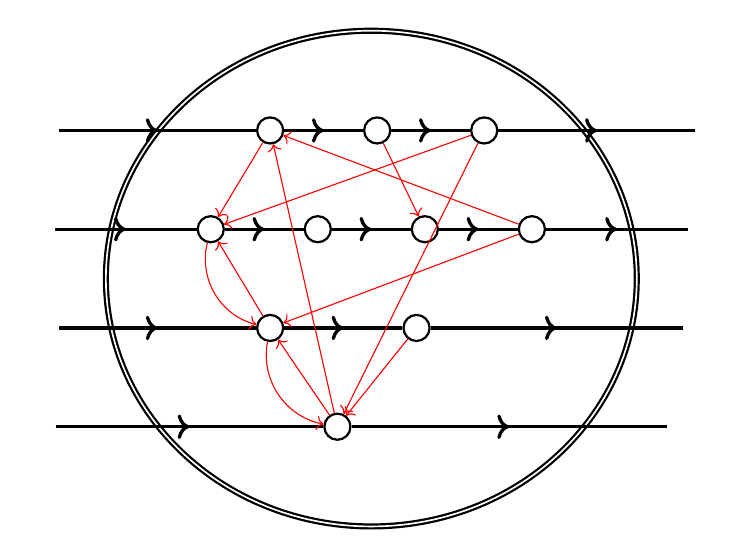
\begin{tikzpicture}[declare function={rr=1+0.1*rnd;}]
    \begin{scope}[every node/.style={circle,thick,draw}]
        %level 1
        \node (level11) {};
        \node[right = of level11] (level12) {};
        \node[right = of level12] (level13) {};
    
        %level 2
        \node[below left = 1cm and 0.5cm of level11] (level21) {};
        \node[right = of level21] (level22) {};
        \node[right = of level22] (level23) {};
        \node[right = of level23] (level24) {};
    
        %level 3
        \node[below right = 1cm and 0.5cm of level21] (level31) {};
        \node[right = 1.5cm of level31] (level32) {};
    
        %level 4
        \node[below right = 1cm and 0.6cm of level31] (level41) {};
    
        \node[draw=black,double,fit=(level11)(level13)(level21)(level24)(level41) ,inner sep=1ex,ellipse] (tmp) {};
    
        \node[draw=none,left = 2.5cm of level11] (level1start) {};
        \node[draw=none,left = 1.8cm of level21] (level2start) {};
        \node[draw=none,left = 2.5cm of level31] (level3start) {};
        \node[draw=none,left = 3.4cm of level41] (level4start) {};
        
        \node[draw=none,right = 2.5cm of level13] (level1end) {};
        \node[draw=none,right = 1.8cm of level24] (level2end) {};
        \node[draw=none,right = 3.2cm of level32] (level3end) {};
        \node[draw=none,right = 4cm of level41] (level4end) {};
    \end{scope}
    
    %blacks
    \begin{scope}[very thick,decoration={
        markings,
        mark=at position 0.5 with {\arrow{>}}}
        ] 
        %level 1
        \draw[postaction={decorate}] (level11)--(level12);
        \draw[postaction={decorate}] (level12)--(level13);
    
        %level 2
        \draw[postaction={decorate}] (level21)--(level22);
        \draw[postaction={decorate}] (level22)--(level23);
        \draw[postaction={decorate}] (level23)--(level24);
    
        %level 3
        \draw[postaction={decorate}] (level31)--(level32);
    
        %start
        \draw[postaction={decorate}] (level1start)--(level11);
        \draw[postaction={decorate}] (level2start)--(level21);
        \draw[postaction={decorate}] (level3start)--(level31);
        \draw[postaction={decorate}] (level4start)--(level41);
        
        %end
        \draw[postaction={decorate}] (level13)--(level1end);
        \draw[postaction={decorate}] (level24)--(level2end);
        \draw[postaction={decorate}] (level32)--(level3end);
        \draw[postaction={decorate}] (level41)--(level4end);
    \end{scope}
    
    %reds
    \begin{scope}
        \path [->,red] (level11) edge node[left] {} (level21);
        \path [->,red] (level12) edge node[left] {} (level23);
        \path [->,red] (level13) edge node[left] {} (level21);
        \path [->,red] (level24) edge node[left] {} (level11);
        \path [->,red] (level31) edge node[left] {} (level21);
        \path [->,red] (level21) edge[bend right=45] node[left] {} (level31);
        \path [->,red] (level31) edge[bend right=45] node[left] {} (level41);
        \path [->,red] (level41) edge node[left] {} (level31);
        \path [->,red] (level32) edge node[left] {} (level41);
        \path [->,red] (level41) edge node[left] {} (level11);
        \path [->,red] (level13) edge node[left] {} (level41);
        \path [->,red] (level24) edge node[left] {} (level31);
    \end{scope}
    \end{tikzpicture}
    \caption{Before path contraction}
    \end{subfigure}
    
    %SECOND
    \begin{subfigure}[b]{1\textwidth}
        \centering
    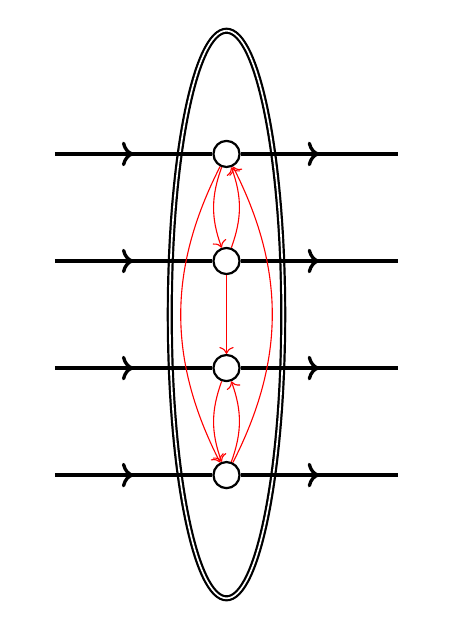
\begin{tikzpicture}[declare function={rr=1+0.1*rnd;}]
        \begin{scope}[every node/.style={circle,thick,draw}]
            %level 1
            \node (level1) {};
        
            %level 2
            \node[below = of level1] (level2) {};
        
            %level 3
            \node[below = of level2] (level3) {};
        
            %level 4
            \node[below = of level3] (level4) {};
        
            \node[draw=black,double,fit=(level1)(level2)(level3)(level4) ,inner sep=2ex,ellipse] (tmp) {};
        
            \node[draw=none,left = 2cm of level1] (level1start) {};
            \node[draw=none,left = 2cm of level2] (level2start) {};
            \node[draw=none,left = 2cm of level3] (level3start) {};
            \node[draw=none,left = 2cm of level4] (level4start) {};
            
            \node[draw=none,right = 2cm of level1] (level1end) {};
            \node[draw=none,right = 2cm of level2] (level2end) {};
            \node[draw=none,right = 2cm of level3] (level3end) {};
            \node[draw=none,right = 2cm of level4] (level4end) {};
        \end{scope}
        
        %blacks
        \begin{scope}[very thick,decoration={
            markings,
            mark=at position 0.5 with {\arrow{>}}}
            ] 
            %start
            \draw[postaction={decorate}] (level1start)--(level1);
            \draw[postaction={decorate}] (level2start)--(level2);
            \draw[postaction={decorate}] (level3start)--(level3);
            \draw[postaction={decorate}] (level4start)--(level4);
            
            %end
            \draw[postaction={decorate}] (level1)--(level1end);
            \draw[postaction={decorate}] (level2)--(level2end);
            \draw[postaction={decorate}] (level3)--(level3end);
            \draw[postaction={decorate}] (level4)--(level4end);
        \end{scope}
        
        %reds
        \begin{scope}
            \path [->,red] (level1) edge[bend right=20] node[left] {} (level2);
            \path [->,red] (level2) edge[bend right=20] node[left] {} (level1);
            \path [->,red] (level2) edge node[left] {} (level3);
            \path [->,red] (level3) edge[bend right=20] node[left] {} (level4);
            \path [->,red] (level4) edge[bend right=20] node[left] {} (level3);
    
            \path [->,red] (level1) edge[bend right=27] node[left] {} (level4);
            \path [->,red] (level4) edge[bend right=27] node[left] {} (level1);
        \end{scope}
    \end{tikzpicture}
    \caption{After path contraction}
    \end{subfigure}
    \caption{}
    \label{fig:contracting}
    \end{figure}
    For all paths in $\mathcal{F}_i$, we make a path contraction (\autoref{fig:contracting}). 
    After contraction or before we delete the remaining arcs if this is done before its the arcs going from the end of a path to a beginning of another path. 
    This action will make $Q_i$ an independent set $\forall i\in [s]$. 
    Since $S$ is a semicomplete digraph, the digraph $D$ would then because of the independence of each $Q_i$ after the path contractions be an extended semicomplete digraph $S'$. 
    Since we have only made path contractions along the cycles in the cycle factor of $D$ and not deleted any arcs that are a part of the cycle factor, $S'$ contains a cycle factor. 
    Then by \autoref{thm:extended}, we know that $S'$ contains a Hamilton cycle. 
    Adding the deleted arcs in each $q_i$ does not change the fact that it contains a Hamilton cycle. We now insert the paths we contracted instead of a node, this makes the cycle longer but it still contains every vertex in the digraph, given a Hamilton cycle in $D$.
\end{proof}

A Hamilton path does not have the same condition for a digraphs to be strong meaning we are also interested in the non-strong quasi-transitive digraphs $T[H_1,\dots ,H_t]$. 
The next theorem is proven in much the same as \autoref{thm:qhcycle}. 
\begin{thm}~\cite{bangJGT20}
    A quasi-transitive digraph $D$ with at least two vertices and with canonical decomposition $D=R[G_1,G_2,\dots , G_r]$ is traceable if and only if it has a $1$-path-cycle factor $\mathcal{F}$ such that no cycle or path of $\mathcal{F}$ is completely in some $D\left< V(G_i)\right>$.
\end{thm}
The proof of \autoref{thm:qhcycle} shows that there is a correlation between the cycle factor of $D$ a quasi-transitive digraph and the path cover of $Q_i$ and therefore we have correlation between the path cover of each $Q_i$ and the hamilton path or cycle. to further explore that we have the following theorem.
but first we need to establish some notation, $pc(D)$ is the path covering number of a digraph $D$. 
\begin{thm}
    Let $D$ be a strong quasi-transitive digraph with canonical decompostion $D=S[Q_1,Q_2,\dots,Q_s]$.
    Let $n_1,\dots n_s$ be the size of the digraphs $Q_1,Q_2,\dots ,Q_s$ respectively. 
    Then $D$ is hamiltonian if and only if the extended semicomplete digraph $S'=S[\overline{K}_{n_1},\dots ,\overline{K}_{n_s}]$ has a cycle subdigraph which covers at least $pc(Q_j)$ vertices of $\overline{K}_{n_j}$ for every $j=1,2,\dots , s$.
\end{thm}
\begin{proof}
    Supose $D$ has a hamilton cycle $H$.
    $V(Q_j)\cap H$ is a $k_j$-path factor $\mathcal{F}_j$ of $Q_j$. 
    $pc(Q_j)$ is the minimum number of path covering $Q_j$ so $k_j\geq pc(Q_j)$. 
    For every $j=1,2,\dots ,s$ we use the path contraction (\autoref{fig:contracting}) of $\mathcal{F}_j$ and delete the remmaining arcs in $Q_j$ results as argued in the proof of \autoref{thm:qhcycle} in a extended semicomplete digraph $S'$ having at least $pc(Q_j)$ vertices in $\overline{K}_{n_j}$ for every $j=1,2,\dots ,s$.\\
    We are now going to show that the other way.
    Suppose $S'$ contains a cycle subdigraph $\mathcal{L}$ containing $p_j\geq pc(Q_j)$ vertices of $\overline{K}_{n_j}$ for every $j=1,2,\dots ,s$.
    By \autoref{thm:5.7.7} $S'$ has a cycle $C$ containing all vertices of the cycle subdigraph $\mathcal{L}$. $V(C)=V(\mathcal{L})$. 
    Hence there is a cycle $C$ covering $p_j$ vertices of each $Q_j$. Since $p_j\geq pc(Q_j)$ there is a $p_j$-path factor in $Q_j$ for every $j=1,2,\dots ,s$.
    We then replace the vertices of $p_j$ of $\overline{K}_{n_j}$ with the $p_j$-path factor in $C$, we do this for all $j=1,2,\dots ,s$ constructing $C'$. Since replacing a vertex in a cycle with a path is still a cycle we have that $C'$ is a cycle and is the hamilton cycle of $D$. 
\end{proof}

We know that the canonical decomposition of a quasi-transitive digraph can be found in polynomial time. 
We can also find the Hamilton cycle in a quasi-transitive digraph in polynomial time, but also verify if it does not exists for the given graph. This result was proved by Gutin. And idear behind it comes from the proof \autoref{thm:notjetstatet} finding the longest cycle in an extended semicomplete digraph from a cycle subdigraph takes time $O(n^3)$ and with the extra operation of finding the coresponding $p_i$-path cover of the houses $Q_i$ we see this is the case.

\begin{thm}~\cite{banggutin94}
    There is an $O(n^4)$ algorithm which, given a quasi-transitive digraph $D$, either returns a Hamiltonian cycle in $D$ or verifies that no such cycle exists.
\end{thm}







	\clearpage
	\part{Linkage and weak linkage}

	\clearpage
	\part{Spanning disjoint subdigraphs (Arc decomposition)}
	\clearpage
\bibliographystyle{unsrt}
\bibliography{bib}
\end{document}